\section{NAND gate}

\subsection{Schematic}

Figure \ref{fig:nand_sch} shows the schematic of a NAND cell, including parameters for MOSFETs.

\begin{figure}[!htb]
	\centering
	\begin{subfigure}[b]{0.55\textwidth}
		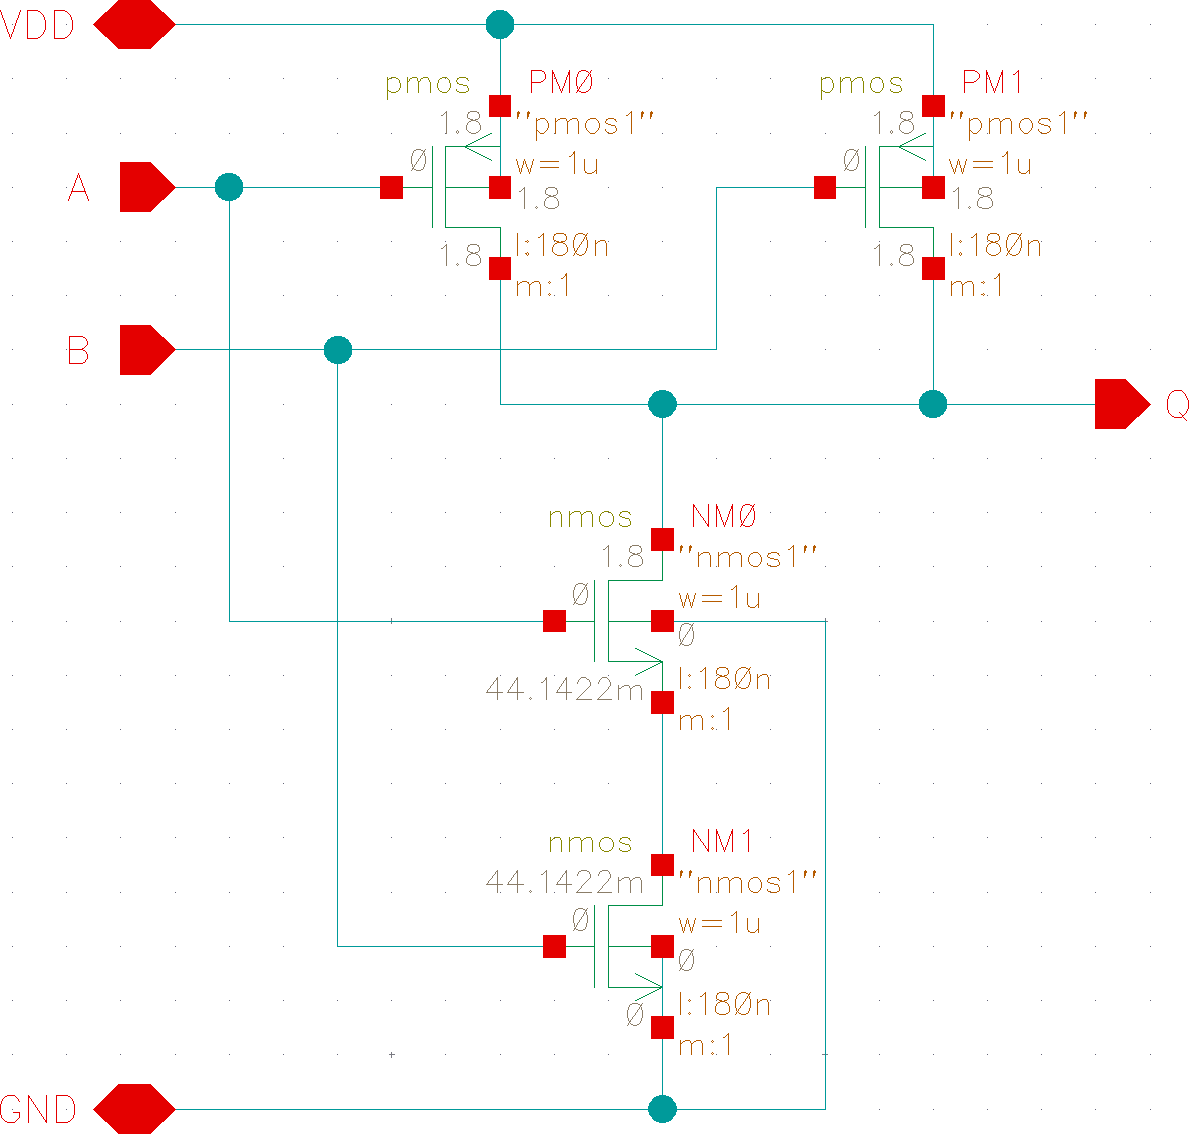
\includegraphics[width=\textwidth]{NAND_sch}
		\caption{Schematic including MOSFET parameters}
		\label{fig:nand_sch}
	\end{subfigure}
	\begin{subfigure}[b]{0.3\textwidth}
		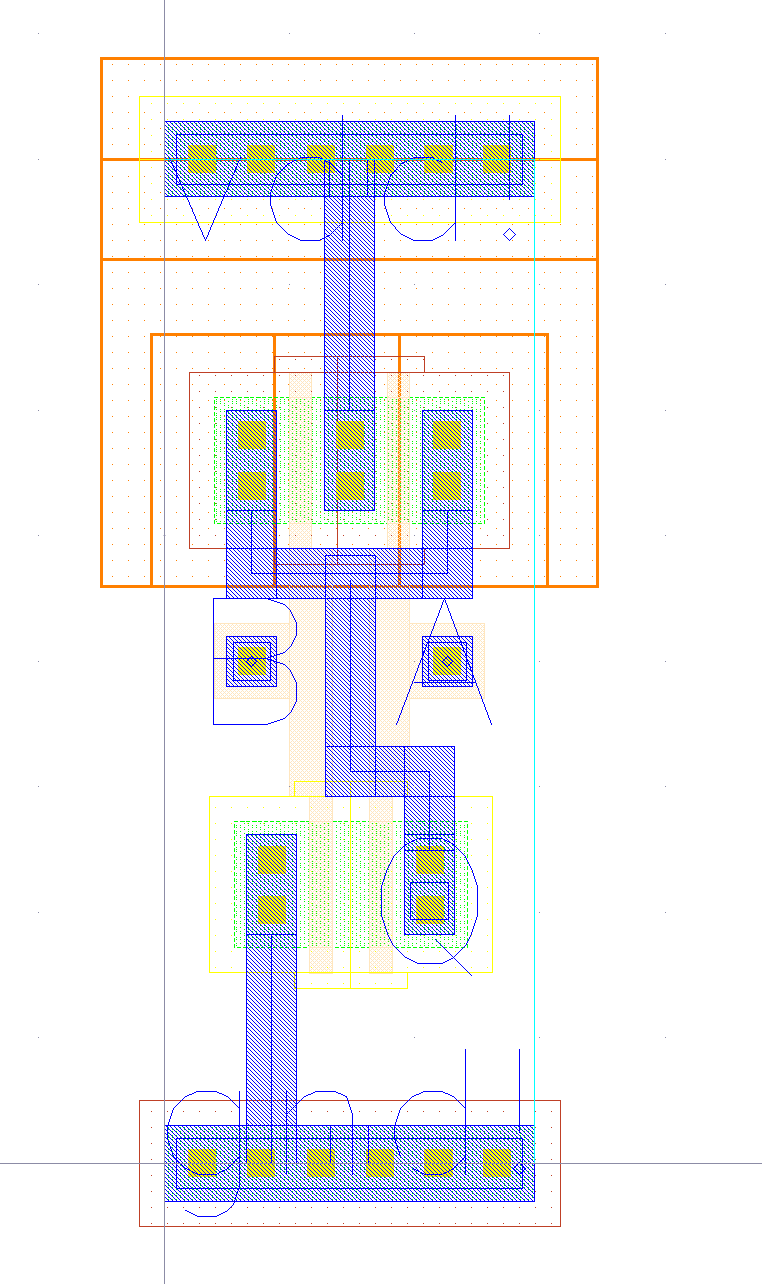
\includegraphics[width=\textwidth]{NAND_lay}
		\caption{Final layout design}
		\label{fig:nand_lay}
	\end{subfigure}
	\caption{A NAND cell}
\end{figure}

\subsection{Determining MOSFET parameters}

According to specification, the NAND gate should be about to drive a $1 pF$ capacitor with a maximum propagation delay of $10 ns$. By applying the time constant equation (Equation \ref{eq:tc}), the resistance for charging the capacitive load should be no more than $10 k \Omega$.

\begin{gather}
	\tau = R C \label{eq:tc} \\
	R = \frac{\tau}{C} = \frac{10 ns}{1 pF} = 10k \Omega \nonumber
\end{gather}

The ON resistances ratio of PMOS and NMOS need to be determined first for transistor sizing. The BSIM3V3 MOSFET simulation models used by the simulator are too complex for direct analysis. Therefore, a simulation of the inverter was used to extract these parameters, as shown in Figure \ref{fig:inv_trans}. The input of the inverter is a square wave with period of $1 \mu s$. The operating points of the circuit were saved every $0.5 \mu s$ after $0.25 \mu s$ into the simulation, when the inverter output is stable. This was done by specifying the logging times in the \texttt{infotime} parameter in the transient simulation options.

\begin{figure}[!htb]
	\centering
	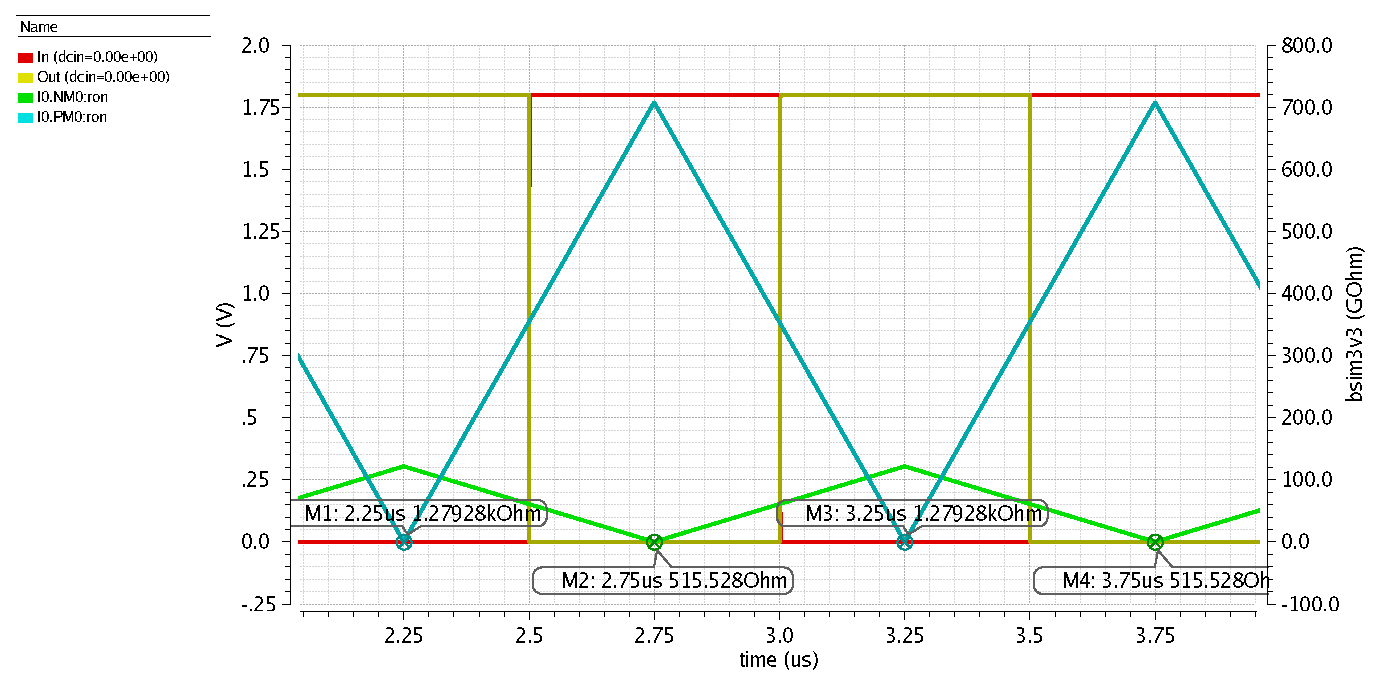
\includegraphics[width=\textwidth]{Inverter_trans}
	\caption{Transient simulation of a Inverter cell with operating points logging}
	\label{fig:inv_trans}
\end{figure}

From the results browser, the ron parameters logged can be plotted with the input and output waveforms. The markers on Figure \ref{fig:inv_trans} shows the ON resistances of PMOS and NMOS transistors, about $1.28 k \Omega$ and $516 \Omega$ respectively. The widths of PMOS and NMOS simulated are $2 \mu m$ and $1 \mu m$ respectively. According to MOSFET modelling (Equation \ref{eq:mosgm}), the ON resistance should be inversely proportional to the width of MOSFETs.

\begin{align}
	%g_m \propto \frac{W}{L} \qquad \text{When $\frac{W}{L}$ variable, $V_{GS} - V_{TH}$ constant}
	g_m = \mu_n C_{ox} \frac{W}{L} (V_{GS} - V_{TH}) \approx \frac{1}{R_{on}}
	%R_o = \frac{1}{2} \mu_n C_{ox} \frac{W}{L} (V_{GS} - V_{TH}) ^ 2
	\label{eq:mosgm}
\end{align}

For balancing the NAND cell, the ON resistances of the PMOS branch and the NMOS branch should be the same. This can be evaluated when both inputs are changing, e.g. from 00 to 11 and from 11 to 00. The output switching point when this is happening should be at half the supply voltage ($1.8 V$), which is about $900 mV$. At this switching point, all PMOS and NMOS transistors are on. By modelling the PMOS and NMOS transistors as resistors of their own ON resistances, the circuit becomes a potential divider, as shown in Figure \ref{fig:nand_model}.

\begin{figure}[!htb]
	\centering
	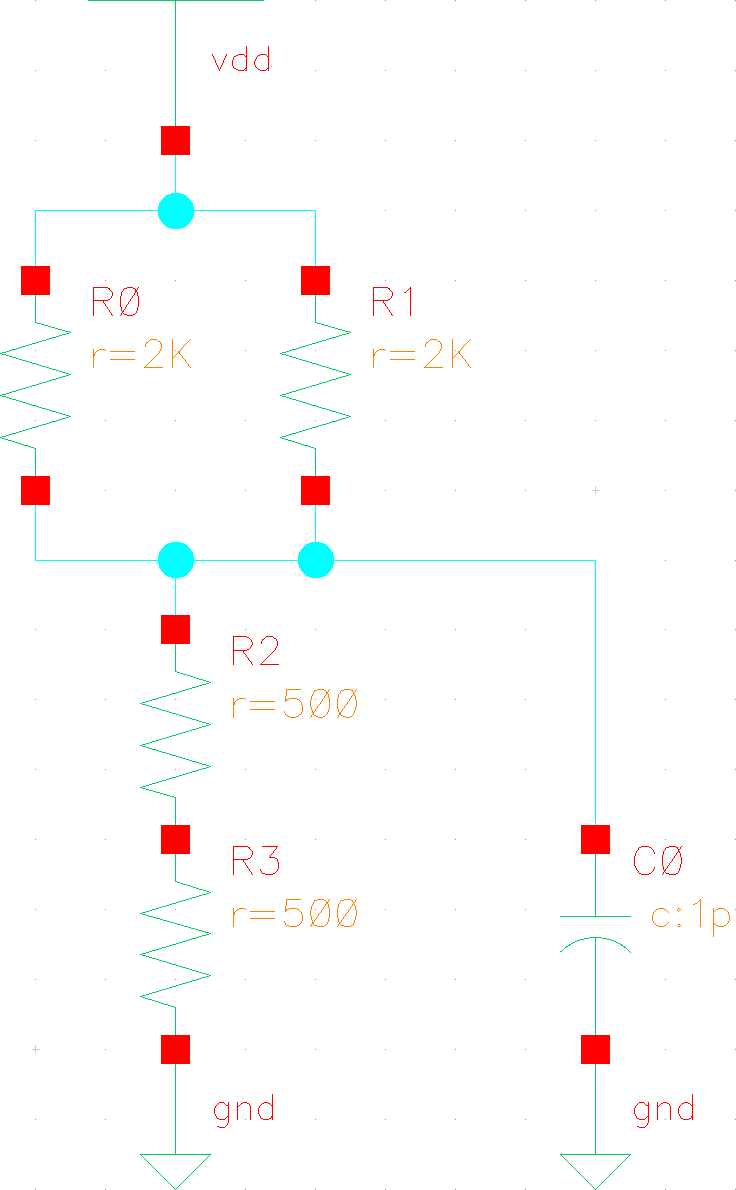
\includegraphics[width=0.3\textwidth]{NAND_model}
	\caption{NAND cell switching point analysis, by modelling MOSFETs as resistors}
	\label{fig:nand_model}
\end{figure}

The widths of NMOS transistors are determined to be $1 \mu m$, the same as the inverter. So the 2 series connected NMOS should add up to a resistance of about $516 \Omega \times 2 = 1.032 k \Omega$. Using a width of $1 \mu m$, a single PMOS will have an ON resistance of approximately $1.28 k \Omega \times 2 = 2.56 k \Omega$. The 2 PMOS transistors are connected in parallel, thus the total resistance of the PMOS branch would be about $\frac{1}{\frac{1}{2.56 k} + \frac{1}{2.56 k}} \Omega = 1.28 k \Omega$. This value is roughly matched with the NMOS branch, and much less than the $10 k \Omega$ value required by the timing specification.

\subsection{Simulation}

Figure \ref{fig:nand_tb_sch} shows the test bench set up for simulating the NAND cell.

\begin{figure}[!htb]
	\centering
	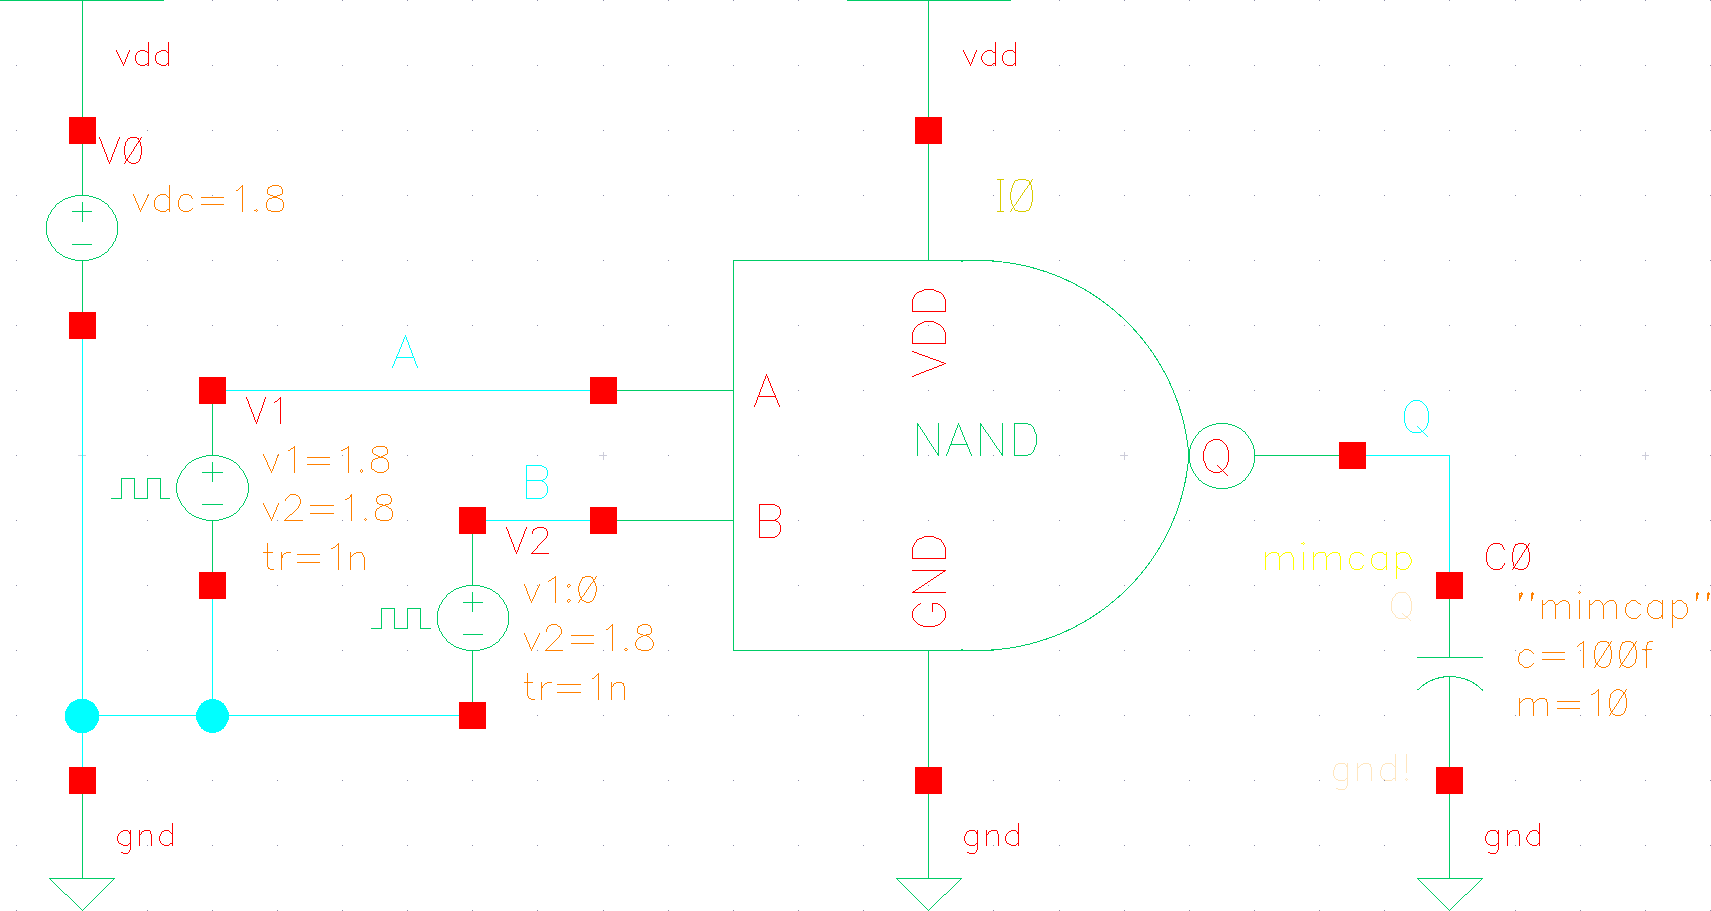
\includegraphics[width=0.7\textwidth]{NAND_tb_sch}
	\caption{NAND simulation test bench set up}
	\label{fig:nand_tb_sch}
\end{figure}

Figure \ref{fig:nand_tb_sim} shows the simulation results for DC sweep and transient analysis.

\begin{figure}[!htb]
	\centering
	\begin{subfigure}[b]{0.45\textwidth}
		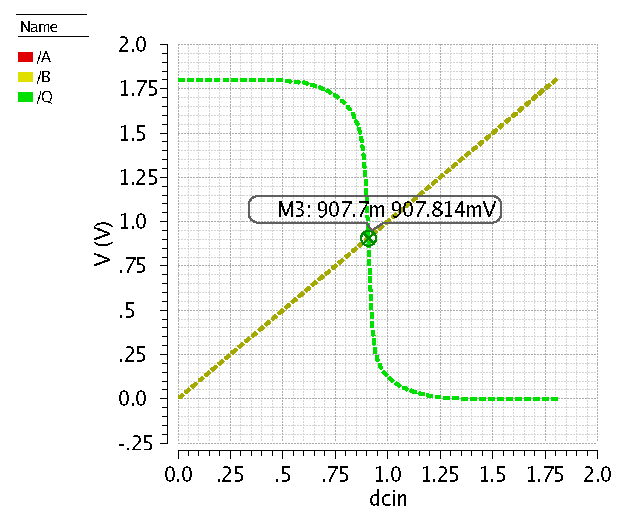
\includegraphics[width=\textwidth]{NAND_tb_dc}
		\caption{DC sweep}
		\label{fig:nand_tb_dc}
	\end{subfigure}
	\begin{subfigure}[b]{0.45\textwidth}
		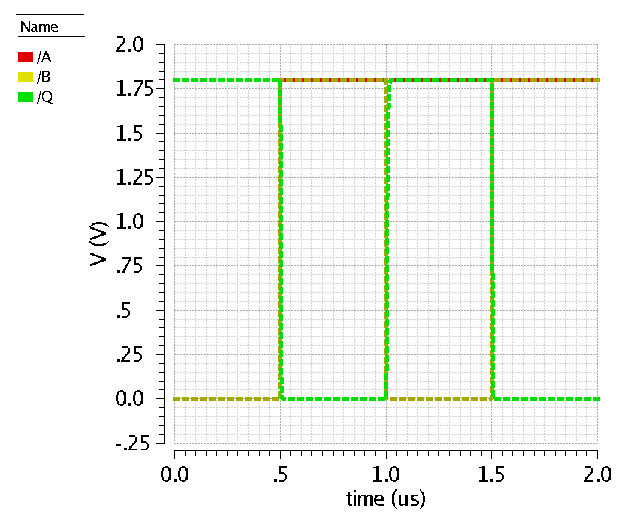
\includegraphics[width=\textwidth]{NAND_tb_trans}
		\caption{Transient}
		\label{fig:nand_tb_trans}
	\end{subfigure}
	\caption{NAND cell simulation}
	\label{fig:nand_tb_sim}
\end{figure}

For DC sweep analysis, both inputs are changing from $0 V$ to $1.8 V$. As the marker suggests, the switching point is about $908 mV$, approximately at half of the power supply. Thus the transistor sizing proposed above do result in a balanced design.

For transient simulation, input A is kept at logic high, only input B is toggling. This gives the worst case propagation delay when output changes from 0 to 1, where only 1 PMOS transistor will be on for driving the output to the required logic level. The close-up of output edges are shown in Figure \ref{fig:nand_tb_edges}. For output rising edge, the output rises to about $1.67 V$ or $93 \%$ in $10 ns$, can be considered within specification.

\begin{figure}[!htb]
	\centering
	\begin{subfigure}[b]{0.45\textwidth}
		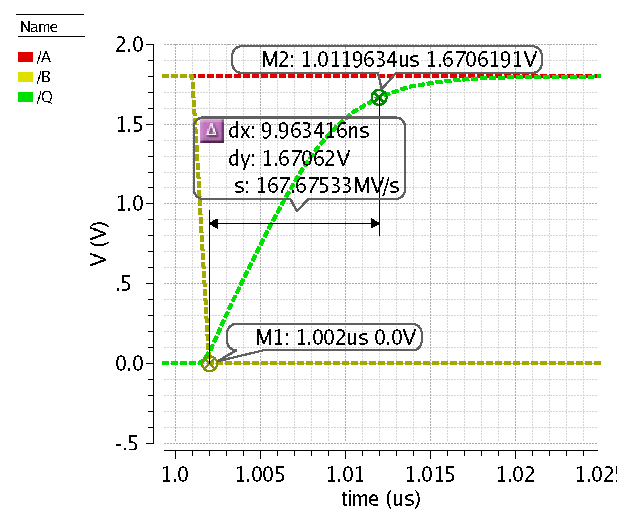
\includegraphics[width=\textwidth]{NAND_tb_rise}
		\caption{Output rising edge}
		\label{fig:nand_tb_rise}
	\end{subfigure}
	\begin{subfigure}[b]{0.45\textwidth}
		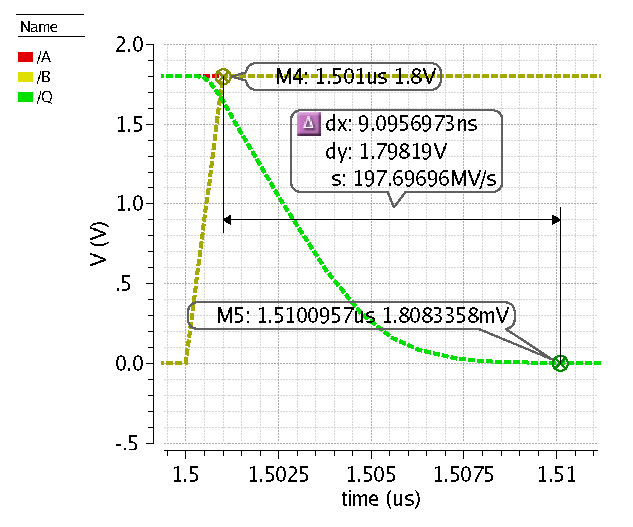
\includegraphics[width=\textwidth]{NAND_tb_fall}
		\caption{Output falling edge}
		\label{fig:nand_tb_fall}
	\end{subfigure}
	\caption{Close-up of transient simulation}
	\label{fig:nand_tb_edges}
\end{figure}

\subsection{Layout}

Figure \ref{fig:nand_lay} shows the final layout designed for the NAND cell. Spacing between P+ implant of the PMOS and cell boundaries is $0.2 \mu m$, as determined earlier during inverter layout design, gives the minimum possible cell width. The 2 PMOS transistors share a common VDD tap, thus can be combined together. The 2 series connected NMOS transistors can also be combined, with no central tap needed. These combinations reduce the cell width a lot, and the layout now looks quite similar to the inverter layout.

This layout design passed the DRC and LVS verification, as shown in Figure \ref{fig:nand_vfy}.

\begin{figure}[!htb]
	\centering
	\begin{subfigure}[b]{0.5\textwidth}
		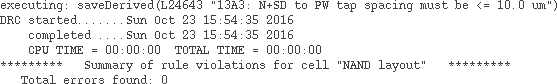
\includegraphics[width=\textwidth]{NAND_drc}
		\caption{DRC checking result, no errors}
		\label{fig:nand_drc}
	\end{subfigure}
	\begin{subfigure}[b]{0.4\textwidth}
		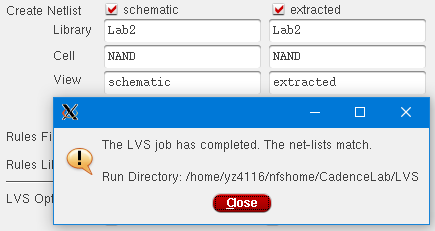
\includegraphics[width=\textwidth]{NAND_lvs}
		\caption{LVS checking result, the extracted net-list matches the schematic}
		\label{fig:nand_lvs}
	\end{subfigure}
	\caption{NAND cell layout verification}
	\label{fig:nand_vfy}
\end{figure}
